
%=========================================================
\chapter{Planeación de Capital Humano}	
\label{cap:capHumano}

	En este capítulo se presenta la planeación del capital humano del proyecto. Se especifican los integrantes, el organigrama, las habilidades de cada integrante, así como sus roles y responsabilidades en el proyecto.

%---------------------------------------------------------
\section{Organigrama}	

\cdtInstrucciones{
	Arme un diagrama jerárquico que capture la cadena de mando o de  información en el proyecto identificando los principales roles en el equipo de trabajo del proyecto.
}

En la figura~\ref{fig:organigrama} se presentan los roles y la cadena de mando en el proyecto. 

\begin{figure}[htbp]
	\begin{center}
		\fbox{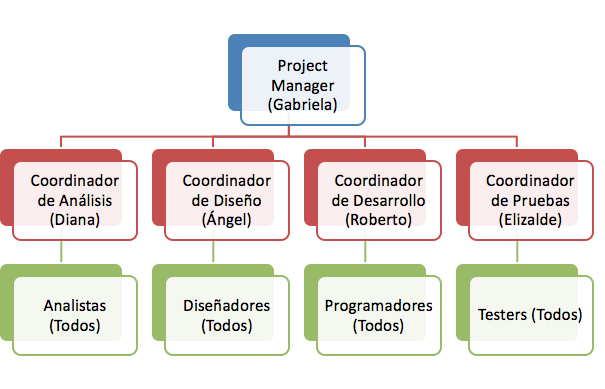
\includegraphics[width=.8\textwidth]{images/Organigrama1}}
		\caption{Organigrama del proyecto}
		\label{fig:organigrama}
	\end{center}
\end{figure}


%---------------------------------------------------------
\section{Responsabilidades}

\cdtInstrucciones{
	Para cada Rol en el proyecto especifique una descripción, responsabilidades dentro del proyecto y habilidades o perfil que se debe cubrir para el puesto.
}


\subsection{Project Manager}
	Líder de proyecto y encargado de el cumplimiento del objetivo del proyecto.
\begin{description}
	\item[Responsabilidades:] \cdtEmpty 	
    \begin{itemize}
    	\item Reconocer los riesgos que puedan impactar la probabilidad de éxito del proyecto.
    	\item Crear políticas para reducir el impacto de los riesgos.
    	\item Planear la ejecución del proyecto en su totalidad.
    	\item Resolver los problemas que se presenten durante la ejecución del proyecto.
    	\item Crear acuerdos entre los coordinadores de las áreas involucradas en el proyecto.
    \end{itemize}
\end{description}

\subsection{Coordinador de Análisis}
	Líder de los analistas y encargado del documento de análisis.
\begin{description}
	\item[Responsabilidades:] \cdtEmpty 	
    \begin{itemize}
    	\item Establecer la forma de trabajo de los analistas y darla a conocer a todo el equipo.
    	\item Asignar tareas a los miembros del equipo de análisis.
    	\item Realizar entrevistas a los usuarios.
    	\item Registrar los tiempos requeridos para realizar las tareas de análisis.
    	\item Realizar el mapeo de procesos.
    	\item Documentar requerimientos.
    	\item Documentar casos de uso.
    	\item Identificar y documentar reglas y términos de negocio.
    	\item Diseñar pantallas.
    	\item Realizar mapas de navegación.
    	\item Responder las dudas en torno al análisis.
    	\item Supervisar el avance del equipo de análisis.
    	\item Establecer acuerdos con el resto de los coordinadores.
    	\item Verificar el trabajo de los analistas.
    	\item Participar en las reuniones de mejora de procesos.
    	\item Documentar lecciones aprendidas.
    \end{itemize}
\end{description}

\subsection{Analista}
	Encargado de realizar el documento de análisis.
\begin{description}
	\item[Responsabilidades:] \cdtEmpty 	
    \begin{itemize}
    	\item Realizar el mapeo de procesos.
    	\item Documentar requerimientos.
    	\item Documentar casos de uso.
    	\item Identificar y documentar reglas y términos de negocio.
    	\item Diseñar pantallas.
    	\item Realizar mapas de navegación.
    	\item Notificar avance al Coordinador de Análisis.
    	\item Notificar cualquier cambio al alcance al Coordinador de Análisis.
    	\item Documentar lecciones aprendidas.
    	\item Participar en las reuniones de mejoras de procesos.
    \end{itemize}
\end{description}

\subsection{Coordinador de diseño}
	Líder de los diseñadores y encargado del documento de diseño.
\begin{description}
	\item[Responsabilidades:] \cdtEmpty 	
    \begin{itemize}
    	\item Establecer la forma de trabajo de los diseñadores y darla a conocer a todo el equipo.
    	\item Planear las actividades de la etapa de diseño.
    	\item Asignar tareas a los miembros del equipo de diseño.
    	\item Traducir los elementos de análisis a en clases y entidades.
    	\item Realizar los diagramas de secuencia para los procesos del sistema.
    	\item Generar el diagrama entidad-relación de la base de datos.
    	\item Responder las dudas en torno al diseño del sistema.
    	\item Supervisar el avance del equipo de diseño.
    	\item Establecer acuerdos con el resto de los coordinadores.
    	\item Verificar el trabajo de los diseñadores.
    	\item Apoyar al arquitecto de software en la definición de la infraestructura.
    	\item Participar en las reuniones de mejora de procesos.
    	\item Registrar los tiempos requeridos para realizar las tareas de diseño.
    	\item Documentar lecciones aprendidas.
    \end{itemize}
\end{description}

\subsection{Diseñador}
	Encargado de realizar el documento de diseño.
\begin{description}
	\item[Responsabilidades:] \cdtEmpty 	
    \begin{itemize}
    	\item Traducir los elementos de análisis en clases y entidades.
    	\item Generar el diagrama entidad-relación de la base de datos.
    	\item Realizar los diagramas de secuencia para los procesos del sistema.
    	\item Informar al Coordinador de Diseño sobre posibles cambios o problemas en la arquitectura del sistema.
    	\item Notificar al Coordinador de Diseño el avance.
    	\item Participar en las reuniones de mejoras de procesos.
    	\item Documentar lecciones aprendidas.
    \end{itemize}
\end{description}

\subsection{Coordinador de desarrollo}
	Líder de los desarrolladores y encargado de la programación del sistema de acuerdo al documento de análisis y diseño.
\begin{description}
	\item[Responsabilidades:] \cdtEmpty 	
    \begin{itemize}
    	\item Establecer la forma de trabajo de los programadores y darla a conocer a todo el equipo.
    	\item Planear las actividades de la etapa de implementación.
    	\item Asignar tareas a los miembros del equipo de desarrollo.
    	\item Implementar los componentes necesarios para los casos de uso asignados, definidos en el diseño.
    	\item Realizar pruebas funcionales sobre los elementos programados.
    	\item Aplicar las buenas prácticas de programación definidas para el proyecto.
    	\item Asegurar la integración de los módulos del sistema.
    	\item Responder las dudas en torno a la programación del sistema.
    	\item Supervisar el avance del equipo de desarrollo.
    	\item Establecer acuerdos con el resto de los coordinadores.
    	\item Verificar el trabajo de los programadores.
    	\item Apoyar al arquitecto de software en la definición de la infraestructura.
    	\item Participar en las reuniones de mejora de procesos.
    	\item Definir la forma de solucionar las incidencias reportadas en la programación.
    	\item Registrar los tiempos requeridos para realizar las tareas de desarrollo.
    	\item Documentar lecciones aprendidas.
    \end{itemize}
\end{description}

\subsection{Programador}
	Encargado de programar el sistema acorde a la documentación.
\begin{description}
	\item[Responsabilidades:] \cdtEmpty 	
    \begin{itemize}
    	\item Implementar los componentes necesarios para los casos de uso asignados, definidos en el diseño.
    	\item Realizar pruebas funcionales sobre los elementos programados.
    	\item Aplicar las buenas prácticas de programación definidas para el proyecto.
    	\item Asegurar la integración de los módulos del sistema.
    	\item Notificar el avance al Coordinador de Programación.
    	\item Participar en las reuniones de mejoras de procesos.
    	\item Documentar lecciones aprendidas.
    \end{itemize}
\end{description}

\subsection{Coordinador de pruebas}
	Líder de los testers y encargado de asegurarse de que el sistema funcione como se estableció en la documentación, y de corrección de errores y bugs.
\begin{description}
	\item[Responsabilidades:] \cdtEmpty 	
    \begin{itemize}
    	\item Establecer la forma de trabajo de los testers y darla a conocer a todo el equipo.
    	\item Planear las actividades de la etapa de pruebas.
    	\item Asignar tareas a los miembros del equipo de pruebas.
    	\item Identificar los escenarios a probar en un caso de uso, módulo o sistema.
    	\item Documentar los guiones de prueba del sistema.
    	\item Documentar los datos de prueba.
    	\item Generar los scripts de prueba para cada escenario.
    	\item Ejecutar las pruebas y documentar los resultados.
    	\item Dar retroalimentación a los programadores sobre los resultados.
    	\item Dar seguimiento a las incidencias encontradas.
    	\item Responder las dudas en torno a las pruebas e incidencias encontradas dentro del sistema.
    	\item Supervisar el avance del equipo de pruebas.
    	\item Supervisar que el proceso de pruebas se realice correctamente.
    	\item Establecer acuerdos con el resto de los coordinadores.
    	\item Verificar el trabajo de los testers.
    	\item Participar en las reuniones de mejora de procesos.
    	\item Registrar los tiempos requeridos para realizar las tareas de pruebas.
    	\item Documentar lecciones aprendidas.
    \end{itemize}
\end{description}

\subsection{Tester}
	Encargado de probar el sistema y reportar el estado de las funciones de éste.
\begin{description}
	\item[Responsabilidades:] \cdtEmpty 	
    \begin{itemize}
    	\item Identificar los escenarios a probar en un caso de uso, módulo o sistema.
    	\item Documentar los guiones de prueba del sistema.
    	\item Documentar los datos de prueba.
    	\item Generar los scripts de prueba para cada escenario.
    	\item Ejecutar las pruebas y documentar los resultados.
    	\item Dar retroalimentación a los programadores sobre los resultados.
    	\item Dar seguimiento a las incidencias encontradas.
    	\item Notificar el avance al Coordinador de Pruebas.
    	\item Notificar al Coordinador de Pruebas de posibles fallos en el análisis o implementación.
    	\item Participar en las reuniones de mejoras de procesos.
    	\item Documentar lecciones aprendidas.
    \end{itemize}
\end{description}

%---------------------------------------------------------
\section{Staff}

\cdtInstrucciones{
	Liste a los integrantes del proyecto especificando su rol, y datos de contacto.\\
}

\begin{table}[hbtp!]
    \noindent\begin{tabular}{|p{.25\textwidth}|p{.15\textwidth}|p{.15\textwidth}|p{.35\textwidth}|}
    	\hline
    	{\bf Nombre} & {\bf Rol} & {\bf Teléfonos} & {\bf Correo}\\
    	\hline
	Moreno González Gabriela & Project Manager & 55 7488 9938 & gonzalez\_gabriela12@hotmail.com \\
        	\hline
    	Mejía Mendoza Diana Laura & Coordinadora de análisis & 55 2034 4711 & dianal\_mm9@hotmail.com \\
    	\hline
	Ferreira Osorno Ángel & Coordinador de diseño & 55 6182 2900 & isc.angel.ipn@gmail.com \\
	\hline
	Mendoza Saavedra Roberto & Coordinador de desarrollo & 55 2184 2095 & isc.robertomendoza@gmail.com \\
	\hline
	Corona Elizalde Luis Ángel & Coordinador de pruebas & 55 1512 1615 & eli17escom@gmail.com \\
    \end{tabular}
	\caption{Integrantes del proyecto.}
	\label{tbl:staff}
\end{table}

